\documentclass{beamer}

\mode<presentation>
{
  \usetheme{CambridgeUS}
  \setbeamercovered{transparent}
}

\usepackage[english]{babel}
\usepackage[latin1]{inputenc}
\usepackage{times}
\usepackage[T1]{fontenc} 
% Or whatever. Note that the encoding and the font should match. If T1
% does not look nice, try deleting the line with the fontenc.
\usepackage{amsmath}

\newcommand{\linespace}{\vskip 0.25cm}

\definecolor{MyForestGreen}{rgb}{0,0.7,0} 
\newcommand{\tableemph}[1]{{#1}}
\newcommand{\tablewin}[1]{\tableemph{#1}}
\newcommand{\tablemid}[1]{\tableemph{#1}}
\newcommand{\tablelose}[1]{\tableemph{#1}}

\definecolor{MyLightGray}{rgb}{0.6,0.6,0.6}
\newcommand{\tabletie}[1]{\color{MyLightGray} {#1}}

% The text in square brackets is the short version of your title and will be used in the
% header/footer depending on your theme.
\title[Developmental plasticity in N-gram GP]{Automating Algorithm Design through\\Genetic Programming Hyper-Heuristics}

% Sub-titles are optional - uncomment and edit the next line if you want one.
% \subtitle{Why does sub-tree crossover work?} 

% The text in square brackets is the short version of your name(s) and will be used in the
% header/footer depending on your theme.
\author[Browning]{Elsa Browning}

% The text in square brackets is the short version of your institution and will be used in the
% header/footer depending on your theme.
\institute[U of Minn, Morris]
{
  Division of Science and Mathematics \\
  University of Minnesota, Morris \\
  Morris, Minnesota, USA
}

% The text in square brackets is the short version of the date if you need that.
\date[April '17] % (optional)
{15 April 2017}

% Delete this, if you do not want the table of contents to pop up at
% the beginning of each subsection:
\AtBeginSection[]
{
  \begin{frame}<beamer>
    \frametitle{Outline}
    \tableofcontents[currentsection, hideothersubsections]
  \end{frame}
}

\begin{document}

\begin{frame}
  \titlepage
\end{frame}

% For a 20-25 minute senior seminar talk you probably want something like:
% - Two or three major sections (other than the summary).
% - At *most* three subsections per section.
% - Talk about 30s to 2min per frame. So there should probably be between
%   15 and 30 frames, all told.

\section*{Overview}

\subsection*{The big picture}

\begin{frame}
  \frametitle{The big picture}
  
  \begin{columns}
  \begin{column}{0.6\textwidth}
  \begin{itemize}
  	\item Developmental plasticity: a powerful source of flexibility in biology
	\item Most EC \& GP systems don't have a developmental phase
	\item Even fewer allow for plasticity during development
	\item N-gram GP has natural developmental phase
	\item Can we add plasticity?
  \end{itemize}
  \end{column}
  \begin{column}{0.4\textwidth}
   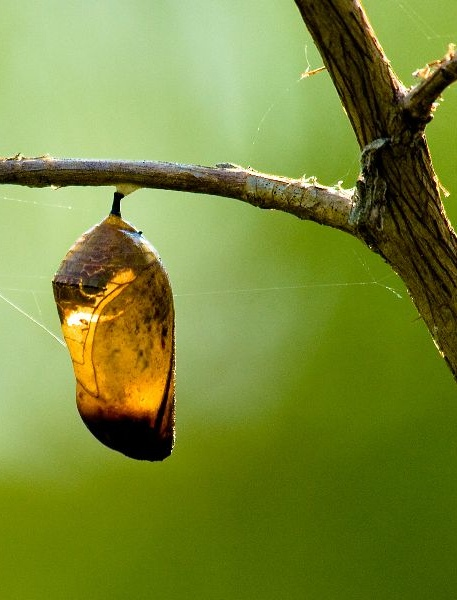
\includegraphics[width=0.95\textwidth]{Illustrations/Empty_cocoon_crop_by_Bluedrakon_from_Flickr.jpg}
       \\
    \only{\tiny{Bluedrakon \\ \url{http://tr.im/pWUi} }}
  \end{column}
  \end{columns}
\end{frame}

\subsection*{Outline}

\begin{frame}
  \frametitle{Outline}
  \tableofcontents[hideallsubsections]
\end{frame}

\section[Developmental plasticity]{Developmental plasticity in biology and EC}

\subsection{Developmental plasticity in biology}

\begin{frame}
  \frametitle{Developmental plasticity in biology}
  
  \begin{columns}
  \begin{column}{.65\textwidth}
Same genome can lead to different physical structures or behavior depending on environmental factors.

\linespace

E.g., color of hornworm caterpillars depends on temperature during development. 

\linespace
  
  Plasticity allows development to respond to environmental changes, adding flexibility.
  \end{column}
  \begin{column}{.35\textwidth}
    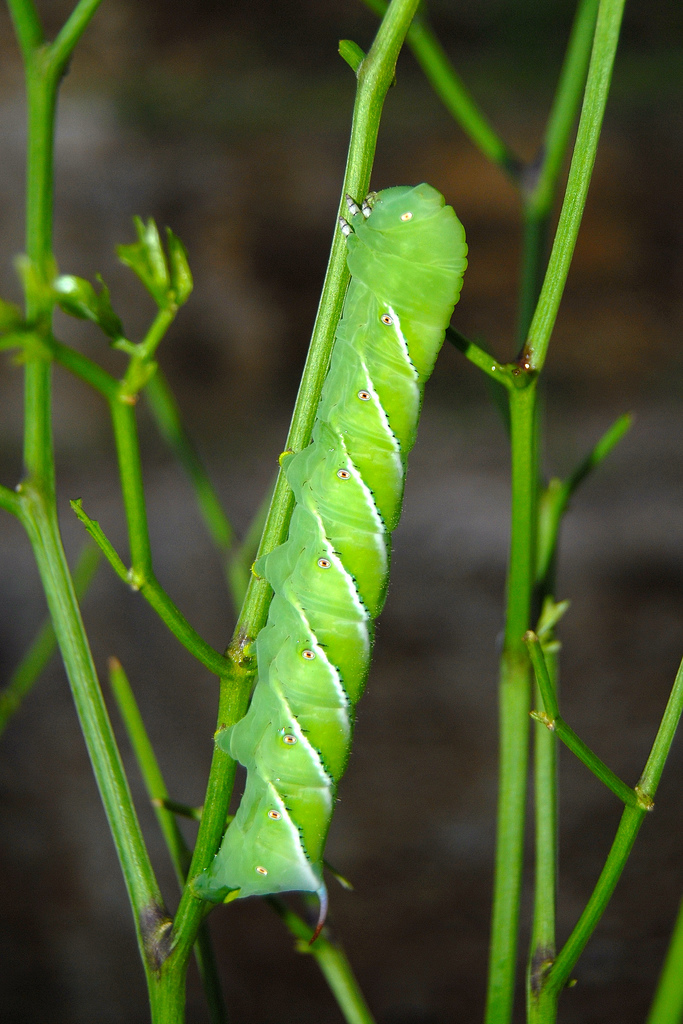
\includegraphics[width=.95\textwidth]{Illustrations/Manduca_sexta_by_Sam_Fraser-Smith_from_Flickr.jpg}
    \\
    \tiny{Sam Fraser-Smith \\ \url{http://tr.im/pq7l} }
  \end{column}
  \end{columns}

\end{frame}

\subsection{Developmental plasticity in EC}

\begin{frame}
	\frametitle{Developmental plasticity in EC}
	
	Most EC systems have no (or trivial) developmental processes.
	\begin{itemize}
		\item Therefore can't have developmental plasticity
	\end{itemize}
	
	\linespace
	
	There are important exceptions.  In GP, e.g.:
	\begin{itemize}
		\item Cellular encoding
		\item Many grammar-based systems
		\item DTAG3P
	\end{itemize}
	
	\linespace 
	
	These remain, however, the exception rather than the rule.
	
	\linespace
	
	N-gram GP has natural developmental process, so a good candidate for adding developmental plasticity.
\end{frame}

\begin{frame}
	\frametitle{Generating programs with N-gram GP}
	
	\begin{columns}
	\begin{column}{0.45\textwidth}
	N-gram GP uses a \emph{probability table} to store likelihood of a triple of instructions appearing in a program:
	\[ Pr\{ x_i \rightarrow x_{i+1} \rightarrow x_{i+2} \}. \]
				
		Given pair of instructions $(x_i, x_{i+1})$, this table gives us the probability distribution for the subsequent instruction $x_{i+2}$.
	\end{column}
	\begin{column}{0.55\textwidth}
	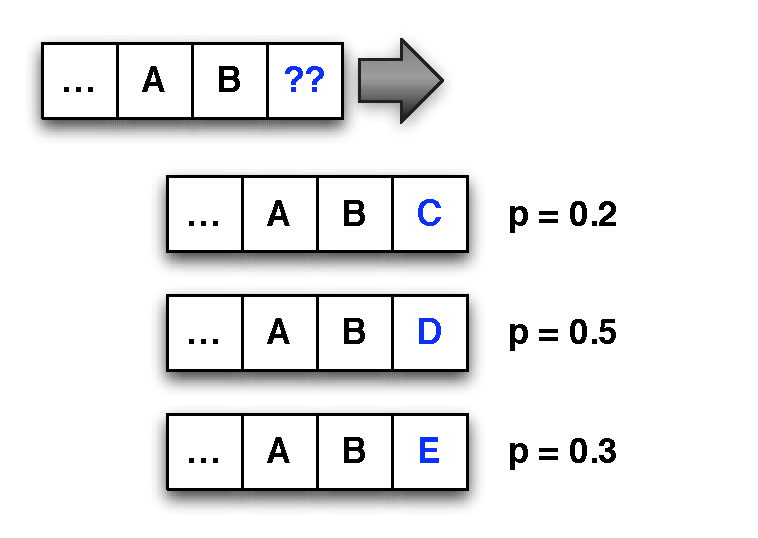
\includegraphics[width=\textwidth]{N_gram_figures/ThreeChoices_v2.pdf}
	\end{column}
	\end{columns}
\end{frame}

\section[Results]{Results}

\subsection[Empirical results]{Empirical comparison of IFD, N-gram GP, and standard GP}

\begin{frame}
  \frametitle{Empirical comparison of IFD, N-gram GP, \& TinyGP}
  
  \begin{columns}[t]
  \begin{column}{0.45\textwidth}
  Compare IFD, regular N-gram GP, and standard sub-tree XO GP (TinyGP)
  \linespace
  \begin{itemize}
	\item 11 different symbolic regression problems
	\item 100 independent runs for each system + problem + parameter set
	\item Various parameter settings (e.g., different block sizes)
  \end{itemize}
  \end{column}

  \begin{column}{0.45\textwidth}
  2 register machine with $+, -, \times$, protected division, and swap
  
  \linespace
  
  Normalize the clock:
  \begin{itemize}
  	\item Count instruction executions
	\item Allow 50M instruction evaluations per run
	\item Store machine state so only new block has to be executed in IFD
  \end{itemize}
  
  \end{column}
  \end{columns}
\end{frame}

\begin{frame}
  \frametitle{Success rates on 11 test problems}
  
\begin{center}
\begin{tabular}{llrrr}
	& & \multicolumn{3}{c}{\emph{Successes out of 100 runs}} \\
	\textbf{Label} & \textbf{Function} & \textbf{TinyGP} & \textbf{N-gram} & \textbf{IFD} \\ \hline
	\tabletie{P1} & \tabletie{$x + x^2 + x^3 + x^4 + x^5$} & \tabletie{100} & \tabletie{100} & \tabletie{100} \\
	\tabletie{P2} & \tabletie{$-x-2x^2+x^3$} & \tabletie{100} & \tabletie{100} & \tabletie{100} \\
	P3 & $1.009 + 1.419x + x^2$ & \tablewin{100} & \tablelose{61} & \tablewin{100} \\
	\tabletie{P4} & \tabletie{$6+x^2+3x^3+8x^5$} & \tabletie{0} & \tabletie{0} & \tabletie{0} \\ \hline
	\tabletie{P5} & \tabletie{$6$} & \tabletie{100} & \tabletie{100} & \tabletie{100} \\ % P4d0f
	P6 & $6+x^2$ & \tablewin{100} & \tablelose{10} & \tablewin{94} \\ % P4d2f
	P7 & $6 + x^2 + 3 x^3$ & \tablewin{85} & \tablelose{0} & \tablelose{1} \\ \hline % P4d3f
	\tabletie{P8} & \tabletie{$8x^5$} & \tabletie{100} & \tabletie{100} & \tabletie{100} \\ % P4d5b
	P9 & $3x^3+8x^5$ & \tablelose{22} & \tablemid{55} & \tablewin{100} \\ % P4d3b
	P10 & $x^2+3x^3+8x^5$ & \tablewin{100} & \tablelose{7} & \tablemid{80} \\ \hline % P4d2b
	Sine & $sin(x)$ & \tablelose{0} & \tablelose{1} & \tablewin{63} \\ \hline
\end{tabular}
\end{center}
\end{frame}

\begin{frame}
\frametitle{IFD wins either way}

\begin{columns}
\begin{column}{0.6\textwidth}

\begin{itemize}
	\item IFD generates low-error individuals from tables evolved with IFD \textbf{and without IFD}.
	\linespace
	\item IFD's local search is valuable in all phases of the process, even if it wasn't used previously.
	\linespace
	\item N-gram GP isn't able to work effectively with the more complex probability tables that IFD generates.
\end{itemize}
\end{column}

\begin{column}{0.02\textwidth}
\end{column}

\begin{column}{0.5\textwidth}

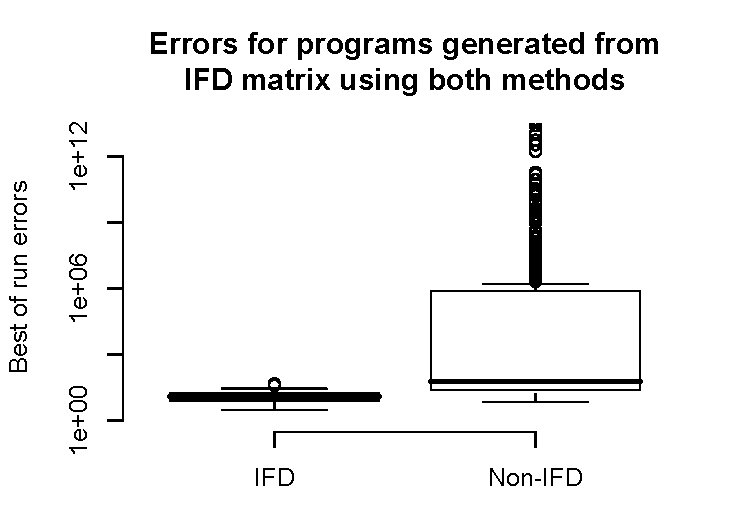
\includegraphics[width=0.915\textwidth]{ErrorsGenedProgsFromIfdMatrix.pdf}

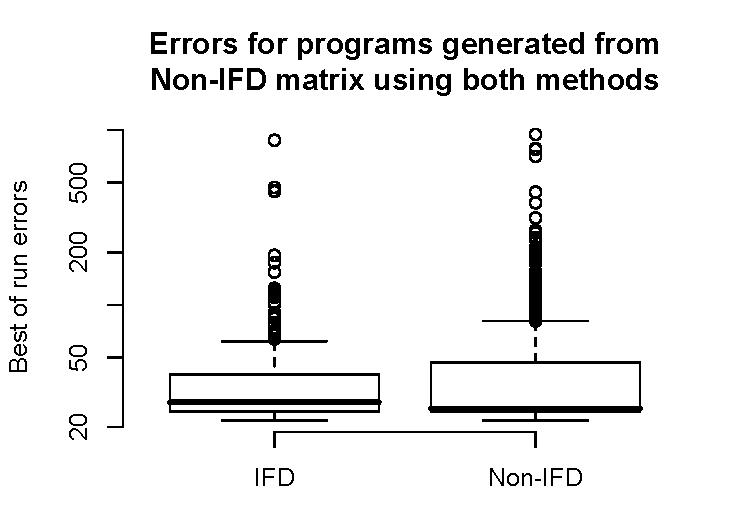
\includegraphics[width=0.915\textwidth]{ErrorsGenedProgsFromNonIfdMatrix.pdf}

\end{column}
\end{columns}

\end{frame}

\subsection[Modularity]{Modularity and repeated structures in IFD}

\begin{frame}
  \frametitle{Structural differences and modularity}
  
  Standard N-gram GP tends to converge to a small set of loops with high probability edges.

  \begin{center}
  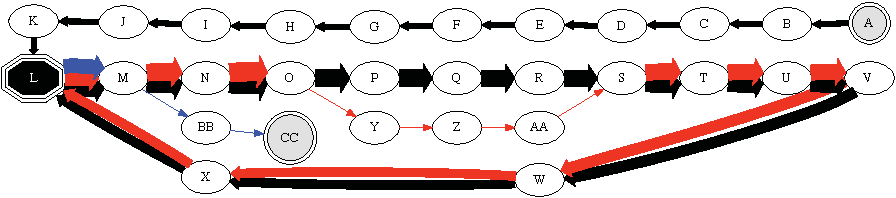
\includegraphics[width=0.8\textwidth]{duplication_graph_40068231_trimmed_smallNodes_coloredEdges_crop.pdf}
  \end{center}
  
      With IFD there is less convergence, more variety and complexity in the modular structure, \& greater use of low probability edges.
  
  \begin{center}
    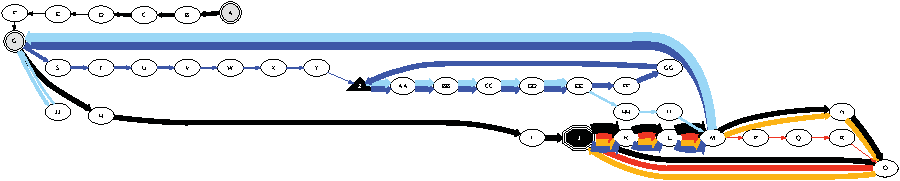
\includegraphics[width=\textwidth]{duplication_graph_12454239_trimmed_smallNodes_coloredEdges_crop.pdf}
    \end{center}

\end{frame}

\section[Conclusions]{Conclusions}

\begin{frame}
\frametitle{Conclusions}

\begin{itemize}
  \item Added developmental plasticity to N-gram GP using Incremental Fitness-based Development (IFD).
\end{itemize}

\begin{itemize}
  \item IFD consistently improved N-gram GP performance on suite of test problems.
  
  \linespace
  
  \item ``Knocking out'' IFD shows it's valuable in all phases, even if it wasn't used earlier in a run.

  \linespace
  
  \item IFD generates more complex, less converged probability tables.
  \item IFD generates more modules/loops \& uses more low-probability paths.
\end{itemize}

\begin{itemize}
  \item Currently exploring applications to dynamic environments.
\end{itemize}

\end{frame}

\begin{frame}
	\frametitle{Thanks!}
	
	Thank you for your time and attention!
		
	\linespace
	\linespace
	
	Contact:  
	\begin{itemize}
		\item \texttt{mcphee@morris.umn.edu}
		\item \url{http://www.morris.umn.edu/~mcphee/}
	\end{itemize}
	
	\linespace
	\linespace
	
	\begin{center}
	{\huge Questions?}
	\end{center}
\end{frame}

\section*{References}

\begin{frame} 
	\frametitle{References} 
	
	\begin{thebibliography}{lskdjf}
	
	\bibitem{McPhee:2009:gecco}
N.~F. McPhee, E.~Crane, S.~Lahr, and R.~Poli.
\newblock Developmental Plasticity in Linear Genetic Programming.
\newblock In G\"unther Raidl, \emph{et al}, editors, {\em GECCO '09}, pages 1019--1026, Montr\'eal, Qu\'ebec, Canada, 2009.
	
	\bibitem{citeulike:3452411}
	R.~Poli and N.~McPhee.
\newblock A linear estimation-of-distribution {GP} system.
\newblock In M.~O'Neill, \emph{et al}, editors, {\em EuroGP 2008}, volume
  4971 of {\em LNCS}, pages 206--217, Naples,
  26-28 Mar. 2008. Springer.
  
  	\end{thebibliography}
	
	\linespace
	\begin{center}
	See the GECCO '09 paper for additional references.
	\end{center}
\end{frame} 

\end{document}


